\documentclass[a4paper]{article}


\usepackage{lipsum}
\usepackage{hyperref}
\usepackage{amsmath}
\usepackage{subcaption}
\usepackage{graphicx}
\usepackage[nottoc,numbib]{tocbibind}


\begin{document}

\begin{titlepage}
	\title{\Huge{Principal Component Analysis}}
	\author{Rajath Kumar M.P. \\ \\  Department of Electronics and Communication Engineering \\ RNS Institute of Technology, Bangalore \\ \\rajathkumar.exe@gmail.com}
	\date{July 21, 2015}
	\maketitle
	\thispagestyle{empty}
\end{titlepage}

\pagenumbering{gobble}
\thispagestyle{empty}
\tableofcontents
\cleardoublepage
\pagenumbering{arabic}


\newpage
\section{Preface}\label{sec:pro}
This paper distills the knowledge on Principal Component Analysis gained after reading about it for a long time now. The concept has been explained in depth mathematically by taking an example.

\section{Introduction}
Principal Component Analysis is the oldest and the most widely used statistical multivariate technique which finds a pattern in the data under consideration. It can be further extended towards dimensionality reduction by extracting important features which are necessary and ignoring the ones which aren't. It find's its application in face recognition, compression, neuroscience etc

\section{One Dimensional Dataset }\label{sec:oned}
\subsection{Mean}
Consider a random one dimensional dataset $X$ with $n$ number of data.
$$X = { 5,2,3,9,1,4 }$$
The mean of $X$ is given by the formula
$${\bar{X} = \frac{ \sum_ {i=1}^n X_i}{n}}$$

Mean gives the center point of the dataset or the average of the entire dataset. Thus the mean, $\bar{X}$ for the considered example dataset will be equal to $4$.
\newline
\parskip 0pt
\\ 
Consider another random one dimensional dataset $Y$
$$Y = { 5,3,2,7,2,5 }$$

The mean, $\bar{Y}$ of this dataset is also $4$. The mean of both the datasets considered are the same but it is clear that the data are different and also it varies differently. The math concept which defines the variation of data is standard deviation.
\subsection{Standard Deviation}
Standard Deviation is a measure that is used to study the amount of variation or dispersion of a set of data values with respect to it's mean. For the $X$ dataset, standard deviation is given by the formula

$$SD = \sqrt{\frac{ \sum_ {i=1}^n {(X_i-\bar{X})^2}}{(n-1)}}$$
$(n-1)$ is Bessel's correction and is applied to yield a better answer.
\subsection{Variance}
Variance is the square of standard deviation.
$$var = SD^2$$
or
$$var={\frac{ \sum_ {i=1}^n {(X_i-\bar{X})^2}}{(n-1)}}$$
\subsection{Conclusion}
The variance of $X$ is 8 and that of  $Y$ is $4$. Which infers that the data of $X$ is more varied or spread across than the data of $Y$.

\section{Two Dimensional Dataset}
Consider a two dimensional dataset, $(X,Y)$

\begin{table}[h!]
\centering
\caption{Two Dimensional Dataset}
\label{tab:xydata}
\begin{tabular}{l c r}\\
$X$ & $Y$ \\ \hline
2 & 1 \\
3 & 4 \\
5 & 8 \\
7 & 7 \\
2 & 1 \\
1 & 3 
\end{tabular}
\end{table}

By applying the same concepts as applied in \ref{sec:oned}, the following results are obtained.\\
\parskip 0pt 
Mean of X,		$\bar{X}$ = 3.3335
\parskip 0pt 
Mean of Y,		$\bar{Y}$ = 4.0
\parskip 0pt 
Variance of X,		$X_{var}$ = 5.0667
\parskip 0pt 
Variance of Y,		$Y_{var}$ = 8.8\\

The above discuss about the dataset itself and not about it's variation or relation with another dataset. The two datasets are compared or analyzed with a parameter called as $Covariance.$
\subsection{Covariance}
Covariance is similar to variance but between two parameters and not with itself. Hence defined as

$$cov(X,Y)={\frac{ \sum_ {i=1}^n {(X_i-\bar{X})}{(Y_i-\bar{Y})}}{(n-1)}}$$
\parskip 0pt 
Rewriting the above formula for $cov(X,X)$ 

$$cov(X,X)={\frac{ \sum_ {i=1}^n {(X_i-\bar{X})}{(X_i-\bar{X})}}{(n-1)}}$$
\parskip 0pt 
or
$$cov(X,X)={\frac{ \sum_ {i=1}^n {(X_i-\bar{X})^2}}{(n-1)}}$$
\parskip 0pt 
which is same as the variance of $X$.\\

For the above considered example the covariance is, $cov(X,Y) = 5.6$\\
The same can be represented in a matrix. This matrix called as the variance-covariance matrix.

\subsection{Variance-Covariance Matrix}

The matrix is depicted as\\

$$\begin{pmatrix} cov(X,X) & cov(X,Y) \\  cov(Y,X) & cov(Y,Y) \end{pmatrix}$$
\parskip 0pt 
Here,\\
\parskip 0pt
$cov(X,X)$ = $X_{var}$\\
\parskip 0pt 
$cov(Y,Y)$ = $Y_{var}$\\
\parskip 0pt 
$cov(X,Y)$ = $cov(Y,X)$\\
\parskip 0pt 
Thus, The variance-covariance matrix can be re-written as

$$\begin{pmatrix} X_{var} & cov(X,Y) \\  cov(X,Y) & Y_{var} \end{pmatrix}$$

Substituting the values as calculated before we get the variance-covariance matrix for the example dataset $(X,Y)$ as

$$\begin{pmatrix} 5.0667 & 5.6 \\  5.6 & 8.8  \end{pmatrix}$$

To extract the principal information content from the datasets or to know which dataset has the most part of information, eigen values and eigen vectors are calculated.

\subsection{Eigen Values and Eigen Vectors}
Consider a set of vectors $\vec{v1}^{\,},\vec{v2}^{\,},\vec{v3}^{\,}...$ which contains a special vector $\vec{v_{e}}^{\,}$ such that when a transformation is applied the vector does not go any changes but is just scaled.

$$T(\vec{v_{e}}^{\,}) = \lambda\times\vec{v_{e}}^{\,}$$

Here $\lambda$ is the scaling factor and is defined as the eigen value. The vector $\vec{v_{e}}^{\,}$ which remains unchanged is the eigen vector.
\parskip 0pt 
For the above example $(X,Y)$, Eigen values are

$$\begin{pmatrix} 1.03041503 \\  12.83625163  \end{pmatrix}$$
\parskip 0pt 
and the eigen vectors are

$$\begin{pmatrix} -0.81124219 & 0.58471028 \\  0.58471028 & 0.81124219  \end{pmatrix}$$
\parskip 0pt 
The two eigen vectors obtained are always perpendicular to one another.

\subsection{Principal Component}
Principal Component is the eigen vector with the highest eigen value of the data under consideration. It can also be understood as the eigen vector which has been scaled more than the other eigen vectors. This forms the basis of PCA.

In the example the second eigen vector becomes the principal component as it has a higher eigen value of $12.83625$ thus we write a feature matrix for the data set containing the eigen vectors in order of higest to lowest importance. Thus,

$$\begin{pmatrix}  0.58471028 & -0.81124219\\   0.81124219 & 0.58471028 \end{pmatrix}$$
This matrix is defined as feature matrix denoted as $featuremat$.
\subsection{Final Transformed Data}

The final transformed dataset is denoted as $Findata$.
The transpose of $feauturemat$ is taken so that the highest eigen vector comes to the first row and the next highest to the second row and so on.
Now $featuremat$ becomes
$$\begin{pmatrix}  0.58471028 & 0.81124219\\   -0.81124219 & 0.58471028 \end{pmatrix}$$

To make the dataset (X,Y) zero mean, we subtract the dataset with their respective mean as shown in $Table$ \ref{table1}
i.e. $X-\bar{X}$ and i.e. $Y-\bar{Y}$
\begin{table}[!htb]
    \begin{minipage}{.5\linewidth}
      \caption{Dataset (X,Y)}
      \centering
        \begin{tabular}{ll}
            $X$ & $Y$ \\ \hline
2 & 1 \\
3 & 4 \\
5 & 8 \\
7 & 7 \\
2 & 1 \\
1 & 3 
        \end{tabular}
    \end{minipage}%
    \begin{minipage}{.5\linewidth}
      \centering
        \caption{Dataset(X,Y) - Mean}\label{table1}
        \begin{tabular}{ll}
           $X$ & $Y$ \\ \hline
-1.33333 & -3 \\
-0.33333 & 0 \\
1.66667 & 4 \\
3.66667 & 3 \\
-1.33333 & -3 \\
-2.33333 & -1 
        \end{tabular}
    \end{minipage} 
\end{table}

\begin{figure}[!htb]
\centering
\begin{minipage}{.5\textwidth}
  \centering
  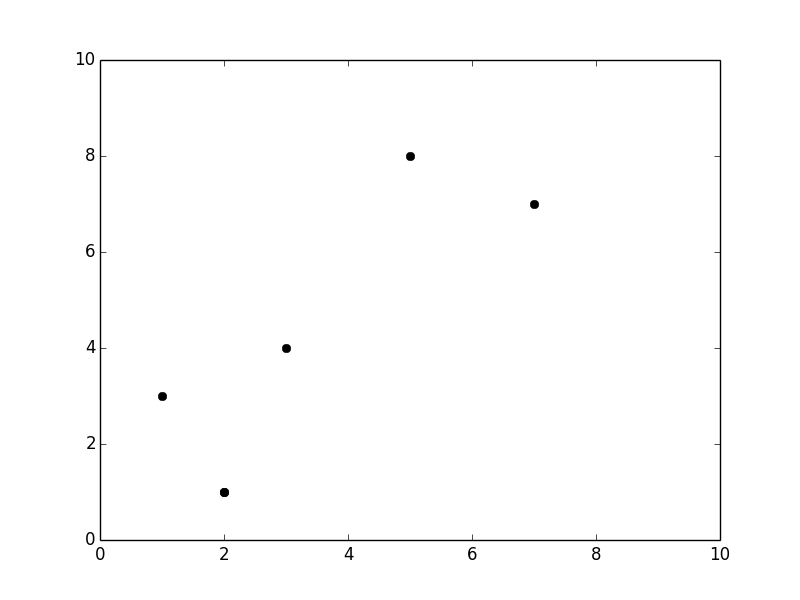
\includegraphics[scale = 0.32]{fig1.png}
  \captionof{figure}{Plot of Dataset(X,Y)}
  \label{fig:test1}
\end{minipage}%
\begin{minipage}{.5\textwidth}
  \centering
  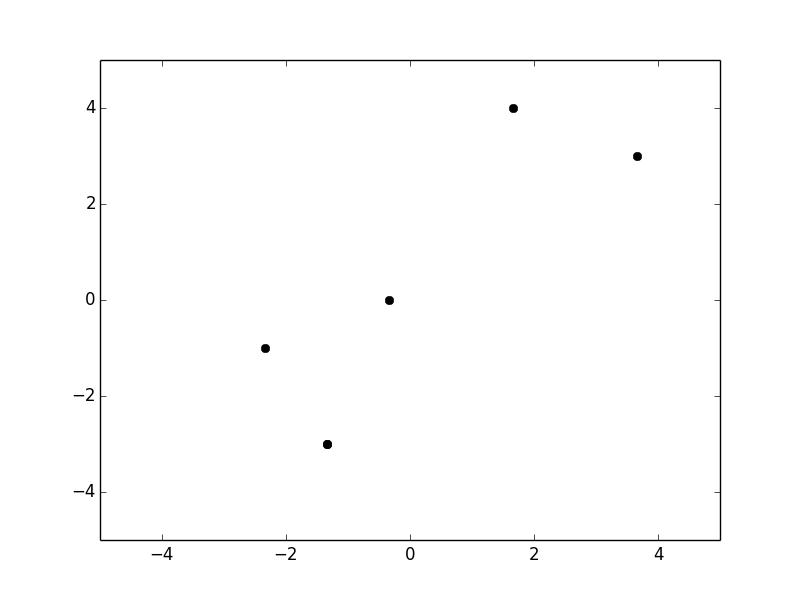
\includegraphics[scale= 0.32]{fig2.png}
  \captionof{figure}{Plot of Dataset(X,Y) - Mean }
  \label{fig:test2}
\end{minipage}
\end{figure}


\begin{figure}[!htbp]
   \centering
   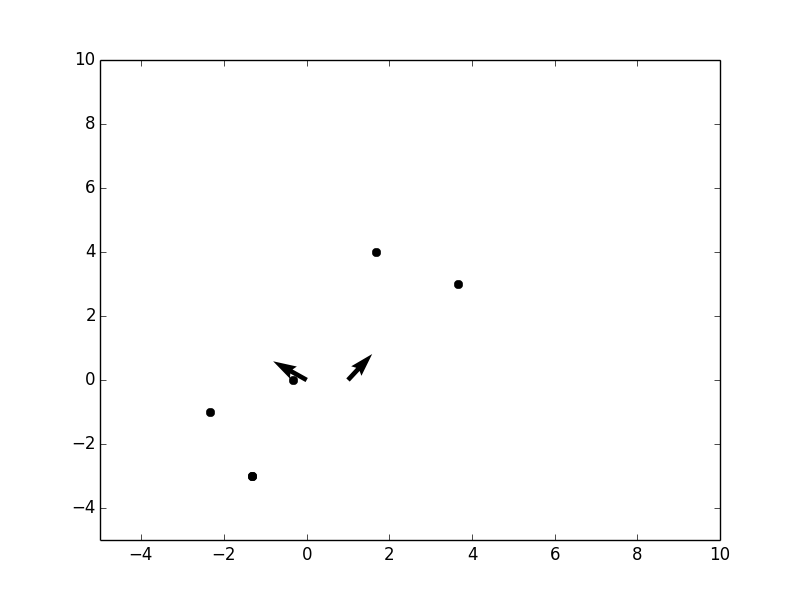
\includegraphics[scale = 0.5]{fig3.png} % requires the graphicx package
   \caption{Plot of Dataset with it's Eigen Vectors}\label{c}
   \label{fig:example}
\end{figure}
\parskip 0pt 
The zero mean dataset obtained is represented in a matrix and denoted as $datam$

$$\begin{pmatrix}
 -1.33333 & -3 \\
-0.33333 & 0 \\
1.66667 & 4 \\
3.66667 & 3 \\
-1.33333 & -3 \\
-2.33333 & -1   \end{pmatrix}$$

The transpose of the $datam$ is taken only if the first column contains the first dataset and second in the second dataset so when transpose is taken first row will have the first dataset, second row the second dataset and so on. Hence taking transpose of $datam$

$$\begin{pmatrix}
 -1.33333 & -0.33333 &1.66667 &3.66667 &-1.33333 &-2.33333 \\ -3 & 0& 4 & 3 &-3 &-1   \end{pmatrix}$$
\parskip 0pt 
The final transformed data is defined as,

$$Findata = featuremat \times datam$$
\parskip 0pt 
Thus we get the final transformed data.
In this case $Findata$ is

$$\begin{pmatrix}-3.2133 & -0.1949 & 4.219 & 4.5777 & -3.2133 & -2.1756\\ -0.6725 & 0.2704 & 0.9868 & -1.2204 & -0.6725 & 1.3082 \end{pmatrix}$$
This is final data obtained. 

\begin{figure}[!htbp]
   \centering
   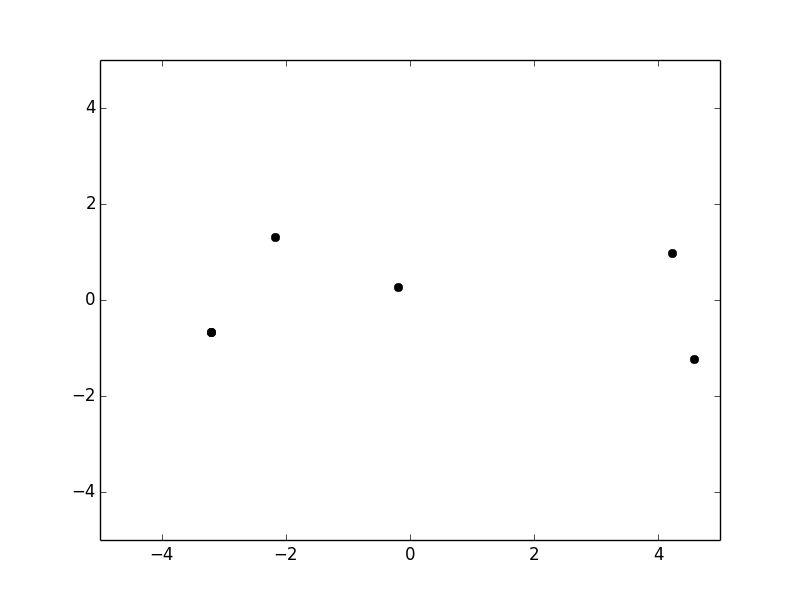
\includegraphics[scale = 0.4]{fig4.png} % requires the graphicx package
   \caption{Plot of Final Transformed Data}\label{ab}
   \label{fig:example3}
\end{figure}

\subsection{Dimensionality Reduction}
To reduce a dimension that is to make a two dimensional data into one dimensional data, The highest eigen vector in the feature matrix is considered and the other eigen vector is ignored and steps are continued by considering only one eigen vector thus the $Findata$ obtained when only the highest eigen vector is considered,

$$\begin{pmatrix}-3.2133 & -0.1949 & 4.219 & 4.5777 & -3.2133 & -2.1756 \end{pmatrix}$$
\parskip 0pt 
This is otherwise called as data reduction or compression.

\subsection{Conclusion}
By comparing the plots \ref{c} and \ref{ab} we can conclude that upon principal component analysis the data set taken into consideration will change its axis into the eigen vector with the highest eigen value this can be observed from the plots. Hence highlighting the highest information content along the axes. Further upon dimensionality reduction the two dimensional dataset changes to one dimensional dataset as only one eigen vector was taken and when plotted the data will be on just one axes or on the eigen vector with the highest eigen value.


\section{Multi Dimensional Dataset}
For Multi dimensional data say $(A,B,C,....)$. Everything is similar to two dimensional dataset but while considering eigenvectors to obtain the final transformed data one has to consider the vectors according to the problem statement or based on the desired reduction in data.

\section{Reconstruction}
To obtain back the original data, $datam$ from the final transformed data the equation 

$$Findata = featuremat \times datam$$

can be rewritten as

$$datam = {featuremat}^{-1} \times Findata$$

$feauturemat$ contains the eigen vectors. If these vectors are unit vectors then the inverse of the matrix is nothing but the transpose of the matrix. But if it is not then the above statement is not true. But in most of the cases the output of most of the math libraries are unit eigen vectors. Now the equation becomes

$$datam = {featuremat}^{T} \times Findata$$
\parskip 0pt 
But $datam$ is zero mean data i.e. mean subtracted data. Hence,

$$datam = Originaldata - Mean$$
\parskip 0pt 
Substituting this in the previous equation

$$Originaldata - Mean = {featuremat}^{-1} \times Findata$$
\parskip 0pt 
Thus $Originaldata$ is expressed as

$$Originaldata = ({featuremat}^{-1} \times Findata) + Mean$$

\bibliographystyle{plain}
\bibliography{pca}

\end{document}